\section{Pourquoi passer à des solutions pair à pair?}
	\label{whyp2p}
	Nous allons savoir pourquoi peut-il être nécessaire dans certains cas, de passer d'une architecture Client/Serveur à une architecture pair à pair, pour cela nous verrons les différences des deux solutions, les avantages et les inconvénients d'une approche pair à pair. Nous avons pu voir qu'il est devenu important, pour les éditeurs de MMOGs, d'étudier les différentes architectures en amont de la réalisation du jeu pour ainsi gérer au mieux les différentes dépenses ~\cite{14101410} (maintenance des serveurs, ajout de add-ons,etc).
	\subsection{Les architectures actuelles pour les MMOGs}
	\par Dans la plupart des jeux en ligne massivement multi joueur, l'architecture est de type client/serveur (voir page~\pageref{P2P/ClServ}). Dans cette architecture, il y a une forte distinction entre le client, qui envoie des requêtes au serveur et attend les réponses, et le serveur qui est à l'écoute de requêtes des clients. Cette approche simplifie la sécurité et le fonctionnent global des jeux. Par exemple, pour effectuer des mises à jour sur l'état global du jeu, il suffit de le faire sur un seule machine (le serveur principal) et il n'y a pas de problème d'incohérence entre les données. De même pour la sécurité, toutes les données étant regroupées sur une seule machine, le contrôle sera beaucoup plus simple que dans des systèmes distribués où le nombre de point d'entrée sera beaucoup plus important. \\
	\par Un des problèmes que peut rencontrer cette architecture est qu'elle aura plus de difficultés pour passer à l'échelle sans mettre de gros moyen en terme de machines et donc financier, le serveur peut devenir un goulot d'étranglement et si un trop grand nombre de joueurs se connecte, le serveur pourrait avoir des difficultés à tenir~\cite{1198269}. Ce problème est résolu en ayant des serveurs de très grandes capacités ou en mettant en place des clusters de serveur. Ces solutions induisent un gros investissement dès le début de la mise en service du jeu et le coût de maintenance est élevé, il est donc difficile de mettre cela en place pour des applications \textit{open source} ou ayant peu de moyen, c'est surtout pour celles-ci que les architectures pair à pair peuvent être intéressantes dans l'immédiat. Un autre problème est la disponibilité du système en cas de panne du serveur, si le serveur tombe en panne alors plus personne n'aura accès à l'application que ce dernier faisait fonctionner, à la différence d'une architecture répartie. \\
	Au vue du nombre croissant de participant à ce genre de jeux vidéos massivement multi joueur, le passage à l'échelle devient un sujet très important et c'est pour cela que les recherches sur des architectures distribuées sont de plus en plus importantes (voir Schéma~\ref{stat_P2P}). \\
	\vspace{5mm} 
        \begin{figure}[!h]
        \centering
        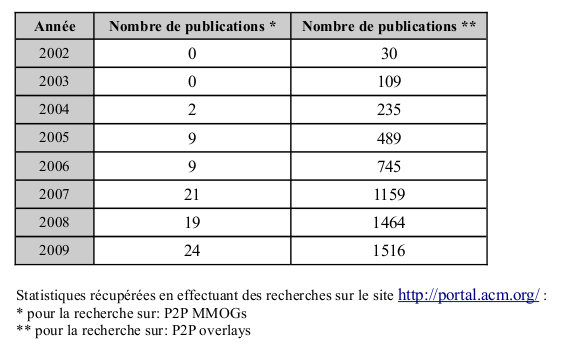
\includegraphics[scale=0.85]{../Images/Stat_Rech_P2P.png}\\
        \caption{Tableau montrant l'évolution des recherches dans le domaine du P2P (MMOGs et Overlay)}
        \label{stat_P2P}
        \end{figure}
	\subsection{Le pair à pair, la solution?}
	\par	%\subsubsection{Avantages}
	Comme il est dit précédemment, l'augmentation croissante des recherches sur le sujet atteste du fait que des problématiques ressortent des solutions existantes. Le problème du passage à l'échelle est sûrement le plus important, et il est l'une des raisons principales de toutes ces recherches. Les architectures pair à pair ne font plus ressortir d'entité serveur et client comme nous le connaissions dans l'architecture client/serveur, chaque nœud sera client et serveur en fonction du temps et en fonction de ses besoins (voir page~\pageref{P2P/ClServ}). Les systèmes pair à pair peuvent avoir une multitude d'utilisation, que ce soit dans le partage de fichier~\cite{gnutella,napster,kazaa}, la communication~\cite{skype}, les jeux vidéos~\cite{starwars}, le calcul scientifique~\cite{Pastry,xtremweb,chord}, le militaire~\cite{jxta}, etc. \\
	\par L'architecture pair à pair est faite telle qu'il n'y a pas de goulot d'étranglement,car nous passons d'un système où tout passait par un point unique à un système qui comporte un grand nombre d'entités qui peuvent toutes avoir le même rôle. L'utilisation de l'architecture pair à pair peut entrainer un grand nombre de communications, elle nécessite des synchronisations des entités, de la gestion des ressources partagées et d'autres problèmes liés à la répartition des données, il faut donc trouver des solutions à tous ces problèmes éventuels. Le pair à pair peut donc être plus adapté, dans certains cas, à des applications massivement multi joueur mais il faudra pouvoir garantir les mêmes propriétés que les systèmes client/serveur. \\
		%\subsubsection{Inconvénients}
	\par Les systèmes pair à pair sont plus difficiles à surveiller, les phénomènes de tricherie sont donc plus difficiles à surveiller, de même pour la sécurité. Nous avons pu voir qu'il existe trois types de tricherie: par Confidentialité, c'est à dire obtenir des informations non autorisées sur d'autres utilisateurs; par Intégrité, si il y des modifications du monde, des lois physiques ou les lois du jeu non autorisées; par Availability, c'est le fait de provoquer des ralentissements ou des arrêts de partie du jeu (référence vers Challenges in P2P gaming). Il faut que le système soit aussi fiable sur le long terme et qu'il soit tolérant aux connexions et déconnexions.\\
	Les jeux vidéos sont des applications distribuées qui ne sont pas dites "critique" (temps réel "mou"), le fait que le jeu ralentisse un petit peu de manière très ponctuelle n'est pas gênant, certaines propriétés des applications distribuées peuvent être retardées ou sautées ponctuellement. Ils ont des avantages qui font qu'il sera moins ardu de réaliser une distribution~\cite{1267692}:
	\begin{itemize}
		\renewcommand{\labelitemi}{$\bullet$}
		\item Les jeux vidéos tolèrent une consistence faible pour les différents états de l'application.
		\item Il peut être possible de prédire les écritures et les lectures grâce à l'ensemble des règles définies dans le jeu. Ce sera le sujet du stage sur l'amélioration de Blue Banana.
	\end{itemize}
	\vspace{1cm}
	\begin{figure}[!h]
	\centering
	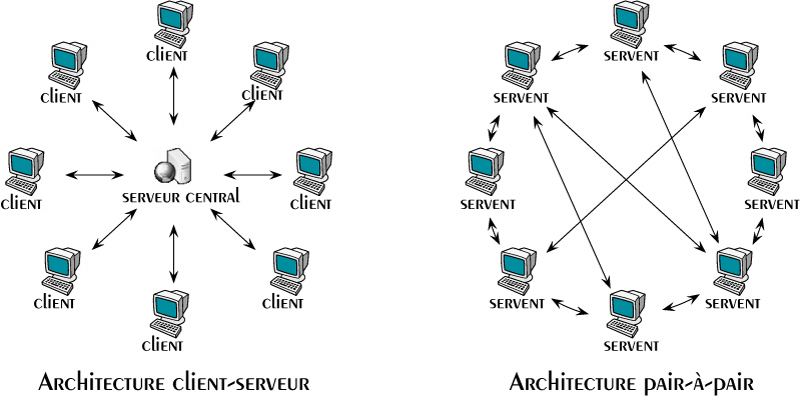
\includegraphics[scale=0.5]{../Images/p2p-85145.png}\\
	\caption{Schéma des architectures pair à pair et client/serveur}
	\label{P2P/ClServ}
	\end{figure} 
\newpage
